
%\usepackage{booktabs}
%\usepackage{textcomp}
%%\usepackage{color}
%%\usepackage{epstopdf}

\documentclass[10pt]{beamer}
%\usepackage[italian]{babel}
\usepackage[USenglish,british,american,australian,english]{babel}
%\usepackage[latin1]{inputenc}
\usepackage[utf8]{inputenc}
\usepackage[T1]{fontenc}
\usepackage{tikz}
\usepackage{bm} % per avere formule in grassetto
%\usepackage[dvips]{graphicx}
\usepackage{xcolor} % formule o testo a colori
\usepackage{indentfirst}
\usepackage{fancyhdr}
\usepackage{fancybox}
\usepackage{graphicx}
%------librerie matematiche-----
\usepackage{amssymb}
\usepackage{amsmath} 
\usepackage{latexsym}
\usepackage{amsthm} 
\usepackage{eucal} 
\usepackage{eufrak}
\usepackage{enumerate}
\usepackage{subfigure}


%--------NEWCOMMAND----

%-- shortcuts for greek letters

\newcommand\eps{\varepsilon}
\newcommand\ph{\varphi}
\newcommand\ka{\kappa}

%\newcommand{\sgn}{sgn}
%\newcommand\ins{}{\{ \}}
%\renewcommand{\ins{}}{\{ \}}
\def \p {{\partial}}
\def \l {{\ell}}

\def \a {{\alpha}}
\def \b {{\beta}}
\def \g {{\gamma}}
\def \d {{\delta}}
\def \la {{\lambda}}
\def \th {{\theta}}

%-- shortcuts for functions
\def \bfA {{\bar{f}^A}}
\def \bfB {{\bar{f}^B}}

\def \hPST {{\hat{\Phi}^{ST}}}
\def \hPAA {{\hat{\Phi}^{AA}}}
\def \hPBB {{\hat{\Phi}^{BB}}}
\def \hPAB {{\hat{\Phi}^{AB}}}
\def \hPBA {{\hat{\Phi}^{BA}}}

%-- shortcuts for operators in macro model
\def \Linkop {{\mathcal{L}}}
\def \Difop {{\mathcal{D}}}
\def \Logop {{\mathcal{R}}}

%-- shortcuts fo the parameters of the model
\def \nucST {{\nu_c^{ST}}}
\def \nucAA {{\nu_c^{AA}}}
\def \nucAB {{\nu_c^{AB}}}
\def \nucBA {{\nu_c^{BA}}}
\def \nucBB {{\nu_c^{BB}}}

\def \nudST {{\nu_d^{ST}}}
\def \nudAA {{\nu_d^{AA}}}
\def \nudAB {{\nu_d^{AB}}}
\def \nudBA {{\nu_d^{BA}}}
\def \nudBB {{\nu_d^{BB}}}

\def \KST {{\kappa^{ST}}}
\def \KAA {{\kappa^{AA}}}
\def \KAB {{\kappa^{AB}}}
\def \KBA {{\kappa^{BA}}}
\def \KBB {{\kappa^{BB}}}

%----------------

%\usepackage{lipsum}

% font-size for selected slides
\newcommand\Fontvi{\fontsize{8}{7.2}\selectfont}
\newcommand\Fontvii{\fontsize{9}{7.2}\selectfont}

% SLIDE 0
%--------------------TITLE PAGE------------------
\title[CEMRACS 2018]{CEMRACS 2018 project:  Mathematical modelling of cell aggregation and segregation.}
%\color{magenta}\shadowbox{Marta Marulli}
%\author[M. Marulli]{Marta Marulli, \\
%\author[1]{Kevin Atsou, Marta Marulli, Rémi Tesson}
%\author[2]{Marta Marulli}
%\author[3]{Rémi Tesson}
%%\author[1]{Static}
%\affil[1]{Laboratoire J.A. Dieudonné, Université de Nice Sophia-Antipolis,}
%\affil[2]{LAGA, Université Paris 13, Università di Bologna,}
%\affil[3]{Institut Mathématiques de Marseille, Aix-Marseille Université}

\author[K.Atsou, M.Marulli, R.Tesson]{Kevin Atsou, \textsuperscript{1} \and Marta Marulli, \inst{2} \and Remi Tesson. \inst{3}}
\institute[]{\textsuperscript{1}  Laboratoire J.A. Dieudonné, Université de Nice Sophia-Antipolis, \and \inst{2} LAGA, Université Paris 13, Università di Bologna, \and \inst{3} Institut Mathématiques de Marseille, Aix-Marseille Université.}



%\textit{in collaboration with}  \\
\date{August 22th 2018}
%\institute{University}
%\logo{\includegraphics[width=15mm]{logo2}}

%------LOGO-----------------------------------------------
\logo{%
  
\includegraphics[width=1.5cm,height=1cm,keepaspectratio]{logo_cirm}}

% beamer theme
\usetheme{Annarbor}
\usecolortheme{lily}

\begin{document}
\begin{frame}
\maketitle
\end{frame}



\section{Introduction}
\begin{frame}
\frametitle{Biological context}
Cell segregation and border sharpening in two-species systems
\begin{figure}[ht]
\centering
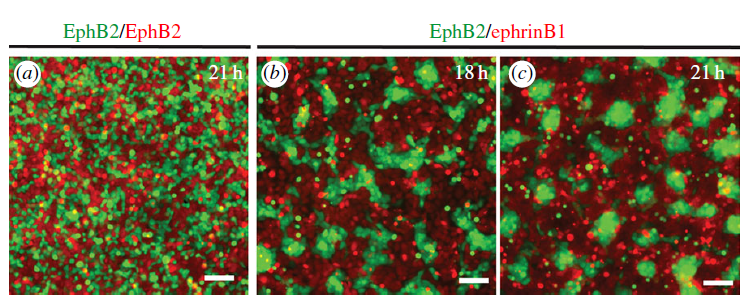
\includegraphics[scale=.6,keepaspectratio]{bio_image}
\end{figure}
\textbf{Working hypothesis:} inter(heterotypic) and intra(homotypic) species repulsion control cell segregation and border sharpening. They have more influence than inter- or intra- species adhesion. 

\textbf{Goal:} to understand the mechanisms of morphogenesis.
\end{frame}


\begin{frame}
\frametitle{blabla}
\end{frame}

\begin{frame}
\frametitle{blabla}
\end{frame}



\section{Mathematical Model}
\begin{frame}
\frametitle{Microscopic framework}
\Fontvii
Individual Based Model for particles interacting through repulsion interactions:
\begin{equation}
	\begin{cases}
d X_i^{A}=-\mu \nabla_{X_{i}^{A}}W^{A}(X^{A},X^{B})dt + \sqrt{2D_{A}} d B_{i}, \quad \forall i \in\{1, \dots, N_{A}\}
\\
d X_i^{B}=-\mu \nabla_{X_{\l}^{A}}W^{B}(X^{A},X^{B})dt + \sqrt{2D_{B}} d B_{\ell}, \quad \forall \l \in \{1, \dots, N_{B}\}
\end{cases}
\end{equation}
where $\mu>0$ is the mobility coefficient and $B_i$ is a 2-dimensional Brownian motion $B_i=(B_i^1,B_i^2)$ of intensity $D_A,D_B>0$ respectively for species A and B.
\end{frame}


\begin{frame}
\frametitle{Macroscopic framework}
\Fontvii
	\begin{equation}
\begin{cases}
\p_t f^{A}=  \nabla \cdot \underbrace{(f^A\nabla_x(\Phi^{AA}* f^A) + f^A \nabla_x( \Phi^{AB}*f^B))}_{interaction \ potential} + \underbrace{ D_A \Delta_x f^A}_{diffusion} + \underbrace{ \textcolor{red}{\nu^{A}f^A\left( 1-\frac{f^A+f^B}{f^{*}} \right)}}_{logistic \ term} \\

\p_t f^{B}=  \nabla \cdot (f^B\nabla_x(\Phi^{BB}* f^B) + f^B \nabla_x (\Phi^{BA}*f^A)) + D_A \Delta_x f^A + \textcolor{red}{\nu^{B}f^B\left( 1-\frac{f^A+f^B}{f^{*}} \right)}
\end{cases}
\end{equation}
with  $f^{S}(x,t)$ particle distributions of type S that give the probability to find a particle of type S at a point $x$ and time $t$, $S \in \{ A,B \}$. \\
 $f^*$: carrying capacity, it represents the maximum popolation size that can be present in the environment.

\end{frame}




\begin{frame}
\frametitle{Macroscopic framework}
\Fontvii
We suppose that the homo-heterotypic species links act as a springs of rest length $R$ between the particles that it is also detection radius  for the interaction.
 \begin{tabular}{cl}  
	\begin{tabular}{c}
		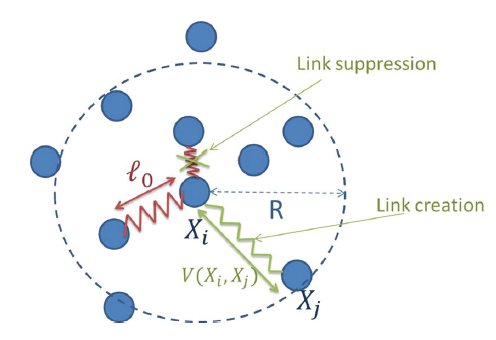
\includegraphics[height=3cm, width=4cm]{link}
	\end{tabular}
	& \begin{tabular}{l}
		\parbox{0.55\linewidth}{%  change the parbox width as appropriate
			\textbf{Case of Hookean springs} \\  
		$$
		\Phi^{ST}(x)=\frac{\nucST}{\nudST}\frac{\KST}{2}
		\begin{cases}
		(|x|-R)^2, \quad \text{for } |x|\leq R\\
		0, \quad \text{for } |x|> R
		\end{cases}
		$$
		with $\nu_{c}^{ST},\nu_{d}^{ST}$ Poisson processes frequencies and $\ka^{ST}$ interaction intensity.
		}
	\end{tabular}  \\
\end{tabular}
$$
pp
$$		
\end{frame}


\begin{frame}
\frametitle{blabla}
\end{frame}


\begin{frame}
\frametitle{Analysis of the macroscopic model}
\Fontvi
	\begin{equation}
\begin{cases}
\p_t f^{A}=  \nabla \cdot (f^A\nabla_x(\Phi^{AA}* f^A) + f^A \nabla_x( \Phi^{AB}*f^B)) + D_A \Delta_x f^A + \textcolor{red}{\nu^{A}f^A\left( 1-\frac{f^A+f^B}{f^{*}} \right)} \\

\p_t f^{B}=  \nabla \cdot (f^B\nabla_x(\Phi^{BB}* f^B) + f^B \nabla_x (\Phi^{BA}*f^A)) + D_A \Delta_x f^A + \textcolor{red}{\nu^{B}f^B\left( 1-\frac{f^A+f^B}{f^{*}} \right)}
\end{cases}
\end{equation}

Linearization around constant steady states $\bfA, \bfB$ and Fourier transform:
\begin{align}
\p_t \begin{pmatrix} \hat{f}^A \\ \hat{f}^B
\end{pmatrix}=
\underbrace{\begin{pmatrix} -|y|^2(2\pi\bfA\hPAA(y)+D_A)-\nu_{b}^A\frac{\bfA}{f^*} & -|y|^22\pi\bfA\hPAB(y)-\nu_{b}^A\frac{\bfA}{f^*} \\ 
-|y|^2\bfB\hPBA(y)-\nu_{b}^B\frac{\bfB}{f^*} & -|y|^2(2\pi\bfB\hPBB(y)+D_B)-\nu_{b}^B\frac{\bfB}{f^*} 
\end{pmatrix}}_{M(y)}
\begin{pmatrix} \hat{f}^A \\ \hat{f}^B
\end{pmatrix}
\end{align}

The constant steady states will be unstable if:
\begin{itemize}
	\item 
	\item 
\end{itemize}

\end{frame}



\begin{frame}
\frametitle{Logistic vs. no logistic}
\begin{columns}[T] % align columns
	\begin{column}{.48\textwidth}
		\color{orange}\rule{\linewidth}{4pt}
		
		Logistic growth model
	\end{column}%
	\hfill%
	\begin{column}{.48\textwidth}
		\color{blue}\rule{\linewidth}{4pt}
		
		No logistic model
	\end{column}%
\end{columns}
\end{frame}




\begin{frame}
\frametitle{Numerical simulations}
\begin{columns}[T] % align columns
	\begin{column}{.48\textwidth}
		\color{orange}\rule{\linewidth}{4pt}
		
		Micro
	\end{column}%
	\hfill%
	\begin{column}{.48\textwidth}
		\color{blue}\rule{\linewidth}{4pt}
		
		Macro
	\end{column}%
\end{columns}
\end{frame}





%\section{Any questions?}
%\begin{frame}
%%\begin{figure}[h]
%%\centering
%%\includegraphics[scale=.2,keepaspectratio]{}
%%\end{figure}
%\end{frame}





\end{document}

